\startchapter{Automated Trojan Detection}
\label{chapter:trojanDetection}

%%%%%%%%%%%%%%%%%%%%%%%%%%%%%%%
\section{Methodology} \label{sec:methodology}
An \acrfull{IC} belongs to one of two categories.
An \acrfull{ASIC} or a \acrfull{FPGA}.
An \acrshort{ASIC} is manufactured once and is immutable; its hardware is permanently printed into its silicon.
\acrshort{FPGA}s are reconfigurable because they are comprised of an array of \acrfull{PLDs}.
A \acrshort{PLD} is a component whose functionality is dependent on a set of configuration options; in other words, a user can define how it behaves.
Each \acrshort{PLD} receives configuration instructions from the user that defines its functionality; these instructions are in the form of a binary message.

The methodology proposed in this chapter focuses on \acrshort{FPGA} devices manufactured by \Xilinx.
In \Xilinx terminology a \acrshort{PLD} is referred to as a tile. 
A single \acrshort{FPGA} can contain hundreds, or even thousands of tiles; a device is usually made up of over a hundred different types.
Different types are used for different functions, such as \acrfull{IO}, Logic, Memory...etc.
The set of messages sent to all of the tiles in the device from the user is referred to as the configuration \gls{Bitstream}. 

\acrshort{FPGA} users create designs using a programming language referred to as a \acrfull{HDL}.
The design is then compiled and synthesized into a configuration \gls{Bitstream} which is then downloaded or "configured" onto the device.
Creating \acrshort{HDL} designs for \acrshort{FPGA}s is considerably cheaper and easier then designing \acrshort{ASIC} chips.
Additionally, if the user wishes to make modifications the design on the device can be updated when out in the field; this is another large advantage over \acrshort{ASIC}s.
Because of this, \acrshort{FPGA}s are becoming the \acrshort{IC} of choice in larger scale productions.
These same features, however, increase their vulnerability to attack.
\begin{figure}[h]
	\centering
	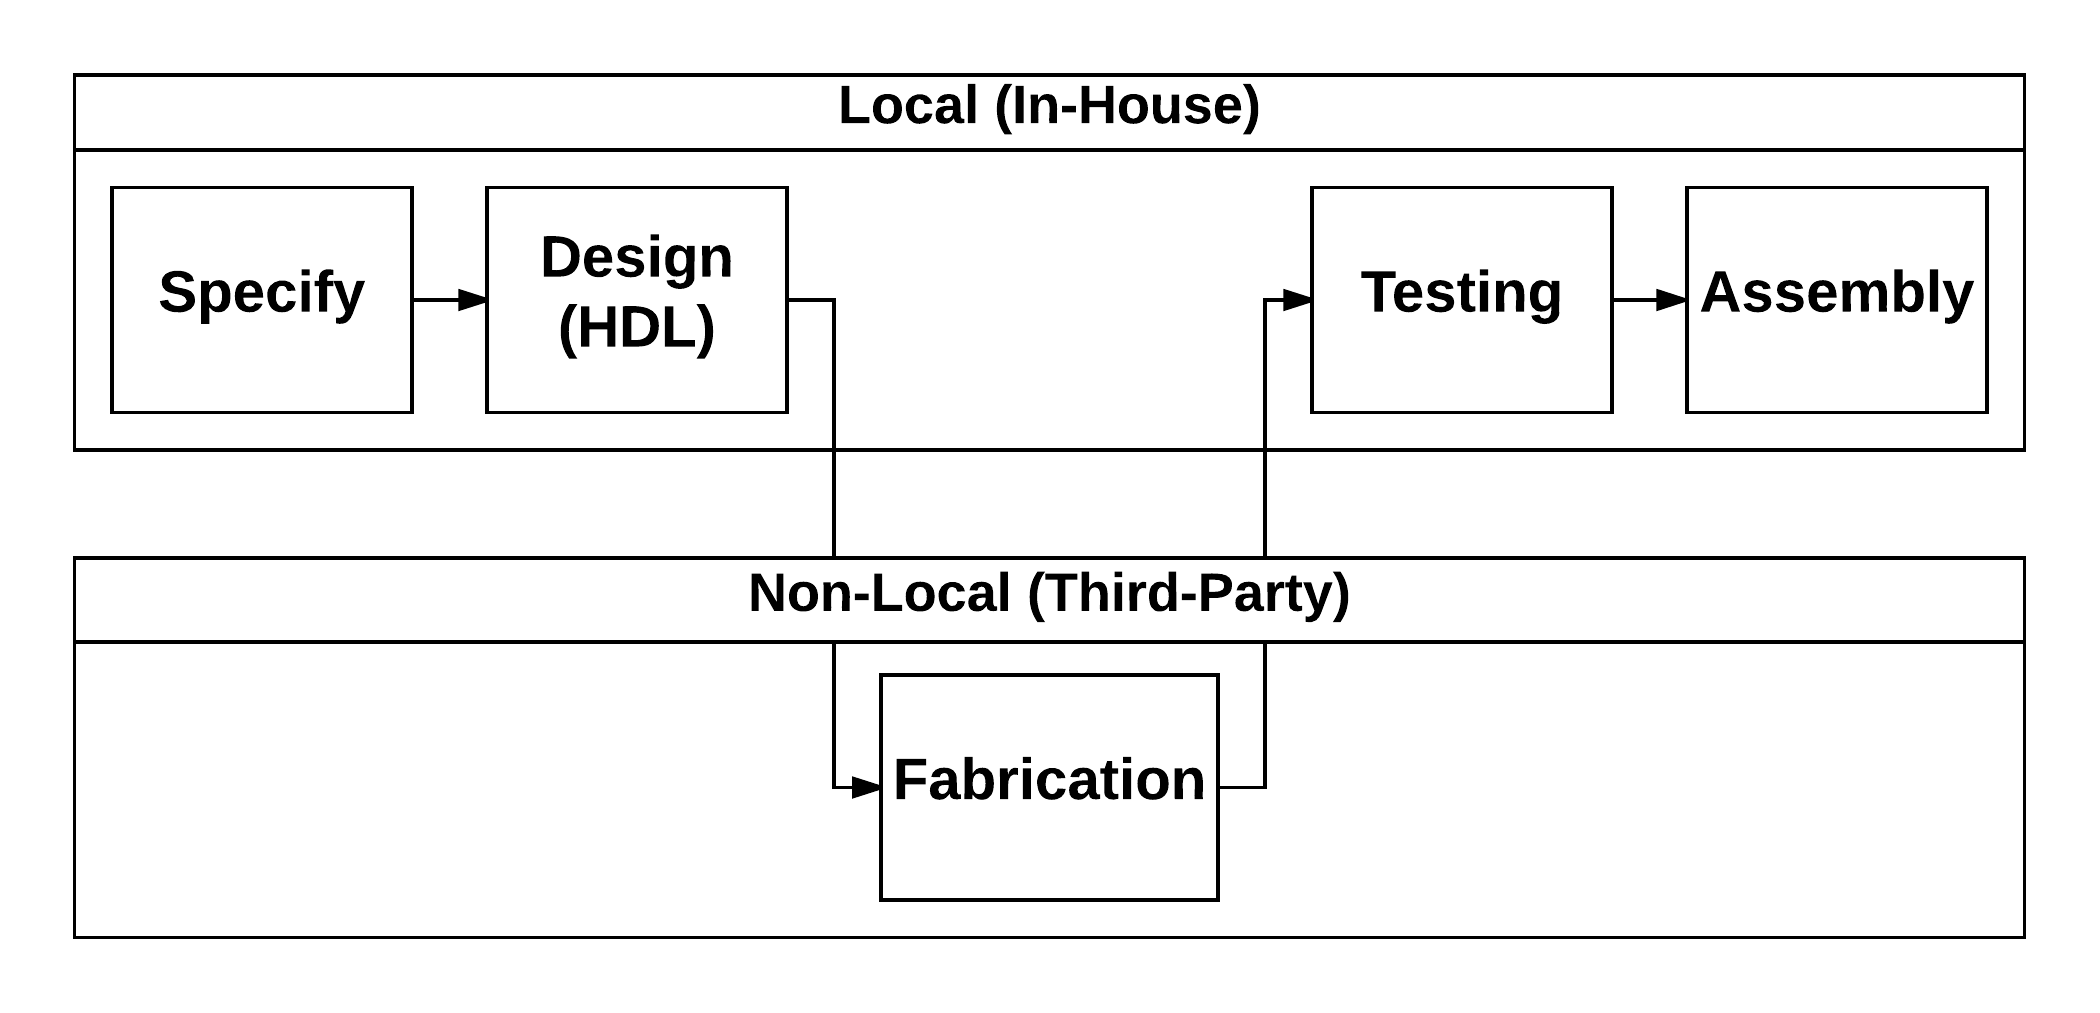
\includegraphics[width=1\linewidth]{figures/Concept}
	\caption[FPGA Life-Cycle]{FPGA Life-Cycle}
	\label{fig:Concept}
\end{figure}

Figure~\ref{fig:Concept} provides a visual representation of the use-case assumed for the purposes of this work. 
With the exception of the fabrication process, all stages of production of an \acrshort{FPGA} implementation are assumed to have been done ``in-house''. 
Any trojan discovered is inserted in the fabrication phase; all other stages are trusted.  
The method of automated trojan detection described in this work would take place in the ``testing'' phase of the life-cycle. 

Figure~\ref{fig:methodologyOverview} shows an overview of the trojan detection methodology.
As mentioned, \acrshort{FPGA} designs are written in a \acrfull{HDL}.
\Xilinx provides a series of \acrfull{UI} and command line tools to process the \acrshort{HDL} known as the ``tool-chain''.
The tool chain generates a series of files that are used for a variety of purposes as shown in the ``Resultant Files'' box in Figure~\ref{fig:methodologyOverview}.
The NGC file is a non-human readable semantic description of the design known as a netlist.
This file can be converted into a human-readable version known as \acrfull{XDL} which will be described in section~\ref{sec:XDL}.
The Bit file is the binary representation of the design to be implemented.
It is referred to as the \gls{Bitstream} or ``configuration'' \gls{Bitstream} and is the final form that is loaded into the \acrshort{FPGA}.
\begin{figure}
	\centering
	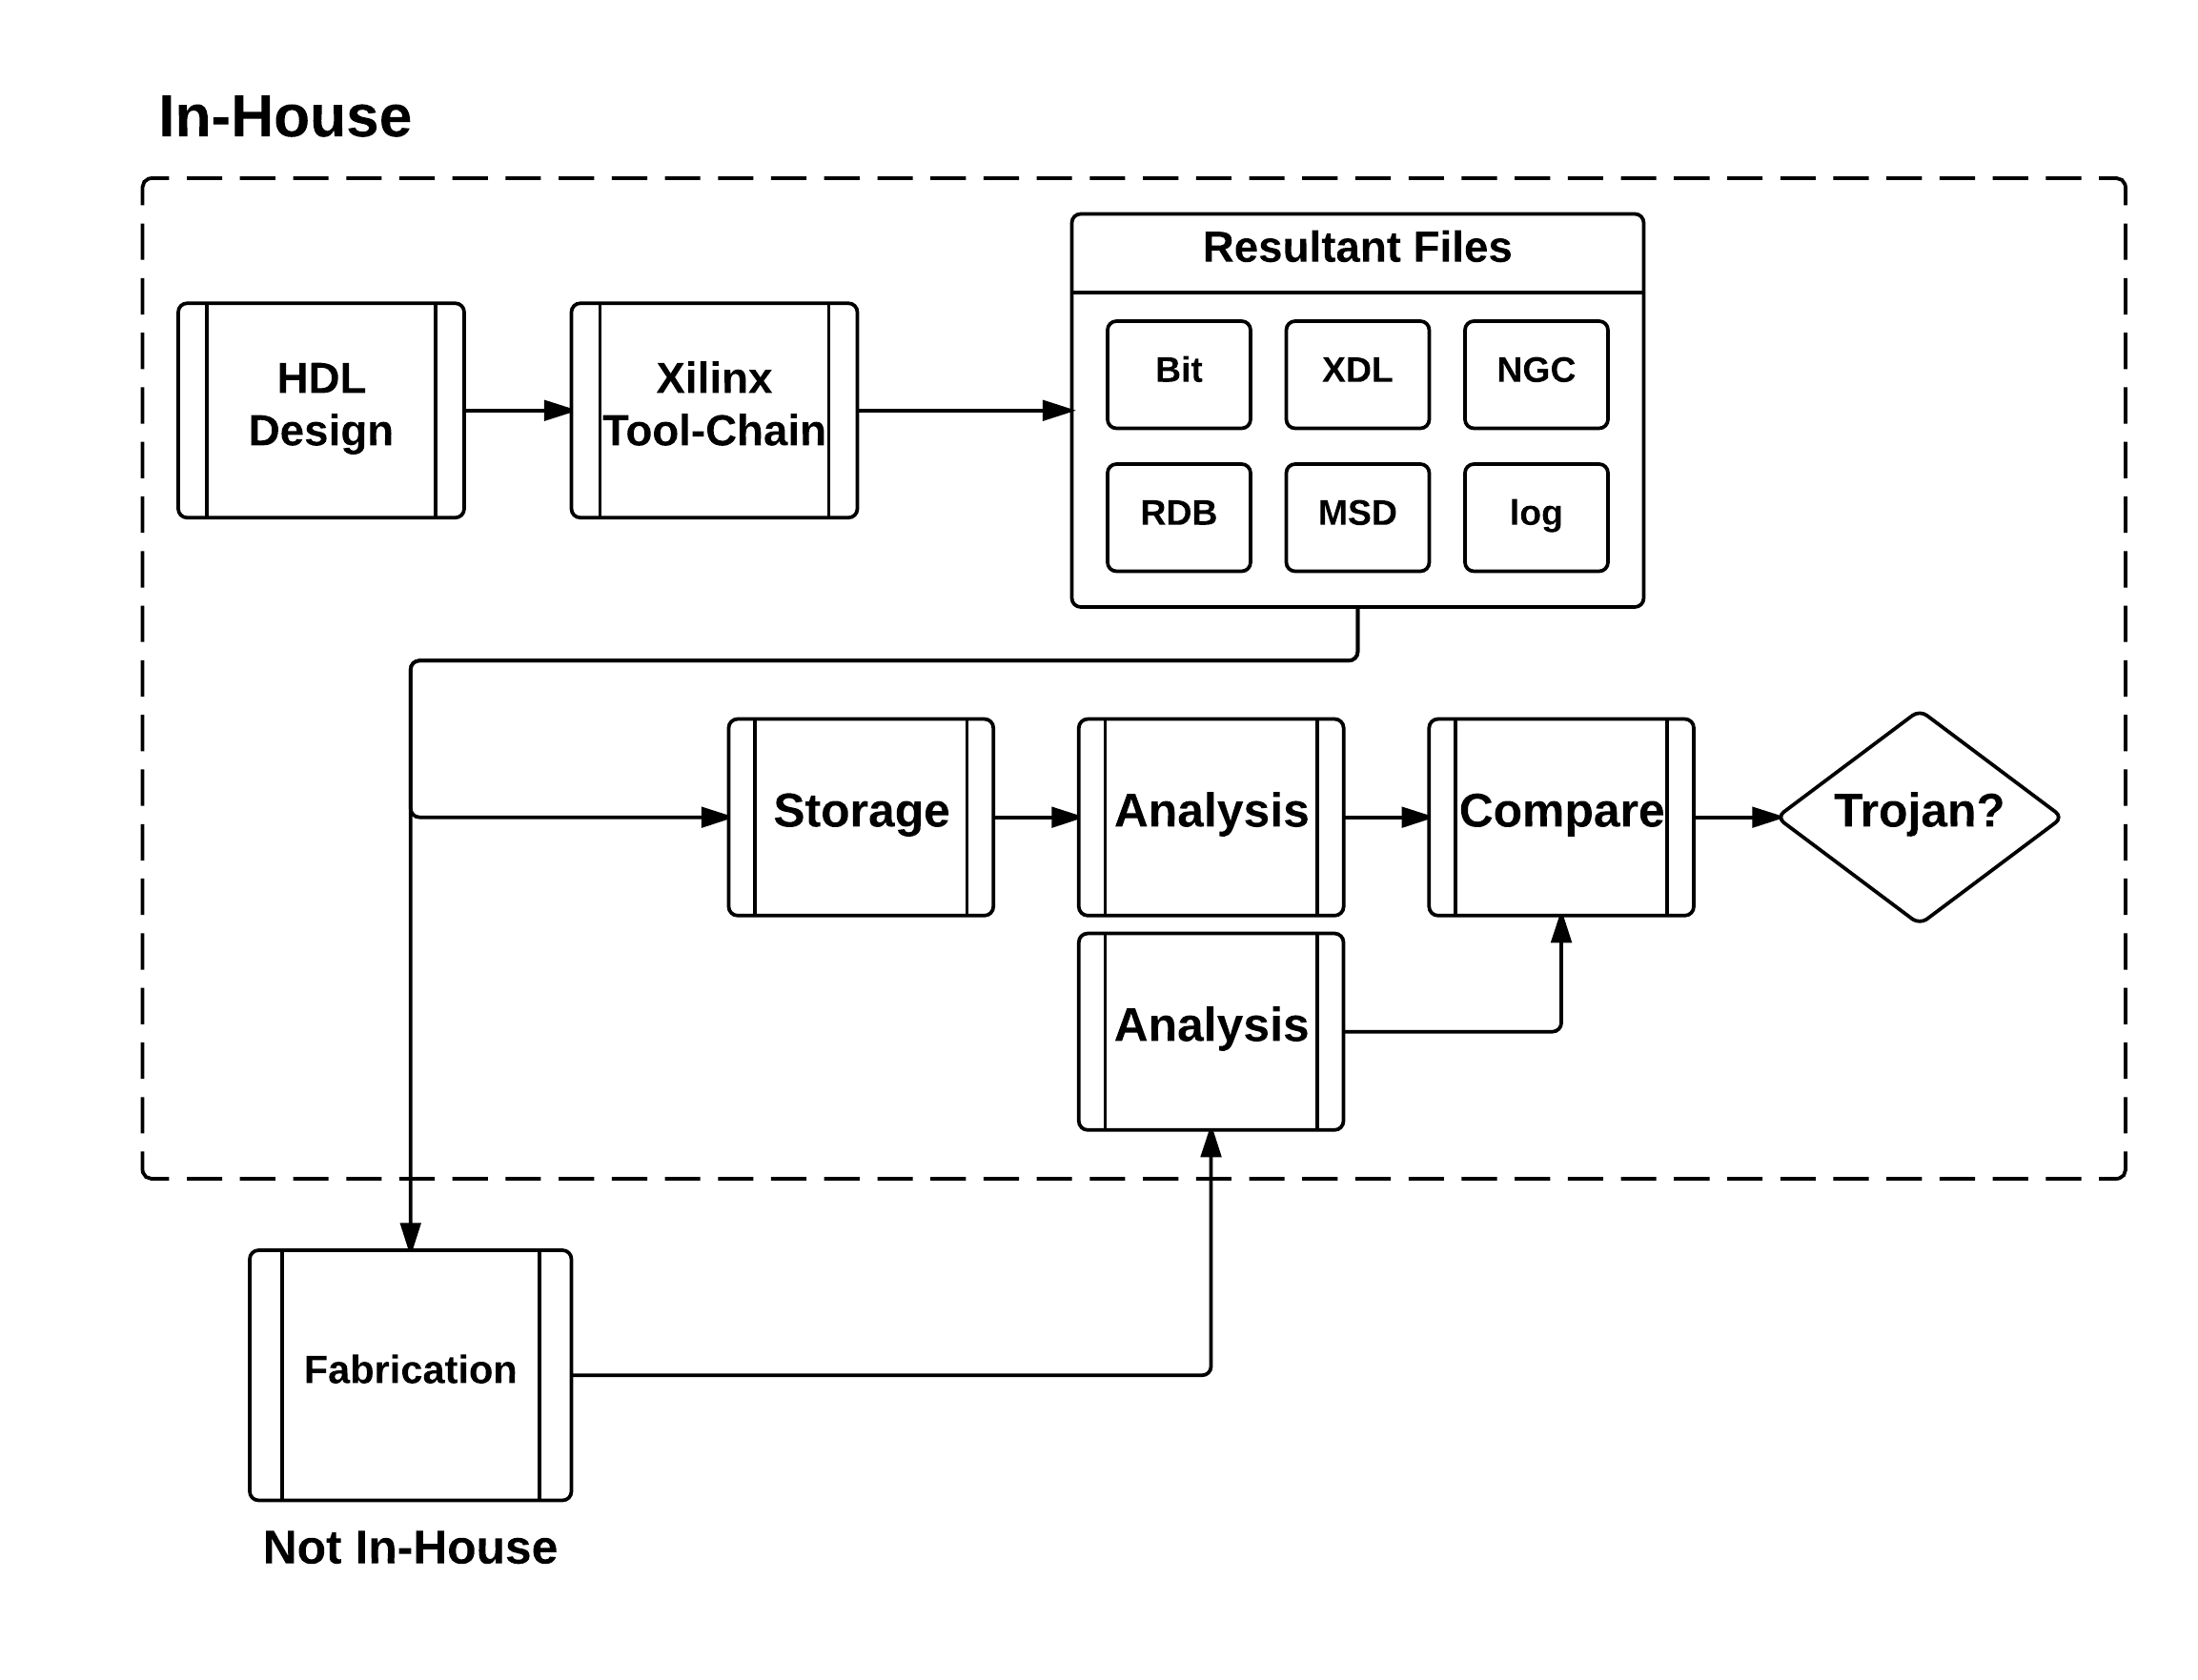
\includegraphics[width=1\linewidth]{Figures/methodologyOverview}
	\caption[Methodology Overview]{Methodology Overview}
	\label{fig:methodologyOverview}
\end{figure}
This Bit file is the primary file sent to the fabrication house where it will be implemented onto the batch of devices ordered.
The resultant files, produced ``in-house'' are to be kept in secure storage while a copy is sent to be fabricated; these stored copies are referred to as \gls{golden} and assumed to be trojan-free.
Though it is known that the fabrication houses will often attempt to make optimizations on designs, this methodology requires that no such efforts be made.
When the completed batch of fabricated chips are returned the \gls{Bitstream} is extracted from a sample via the method described in section~\ref{sec:bitstreamExtraction}. 
That which is extracted is referred to as the \gls{target} \gls{Bitstream}.
The \gls{golden} and \gls{target} \gls{Bitstream}s are analyzed in conjunction to detect differences.
This technique is described in section~\ref{sec:fpgaBitStream}.
Any discovered differences are then attributed to the corresponding component in the architecture, described in section~\ref{sec:tileMapping}.
Finally, the descriptive attributes, originally presented in section~\ref{sec:topology}, are returned to the user.
This is described in section~\ref{sec:trojanAttributes}. 


%%%%%%%%%%%%%%%%%%%%%%%%%%%%%%%
\section{FPGA Architecture and Configuration} \label{sec:architectureAndConfig}
A \Xilinx \acrfull{FPGA} is comprised of a matrix of blocks referred to as the ``gate-array'' and is shown in Figure~\ref{fig:FPGA}~\cite{xilnxDevManual}.
A device can contain anywhere from a couple hundred to a few thousand blocks and are arranged into columns by type.
\begin{figure}[h]
	\centering
	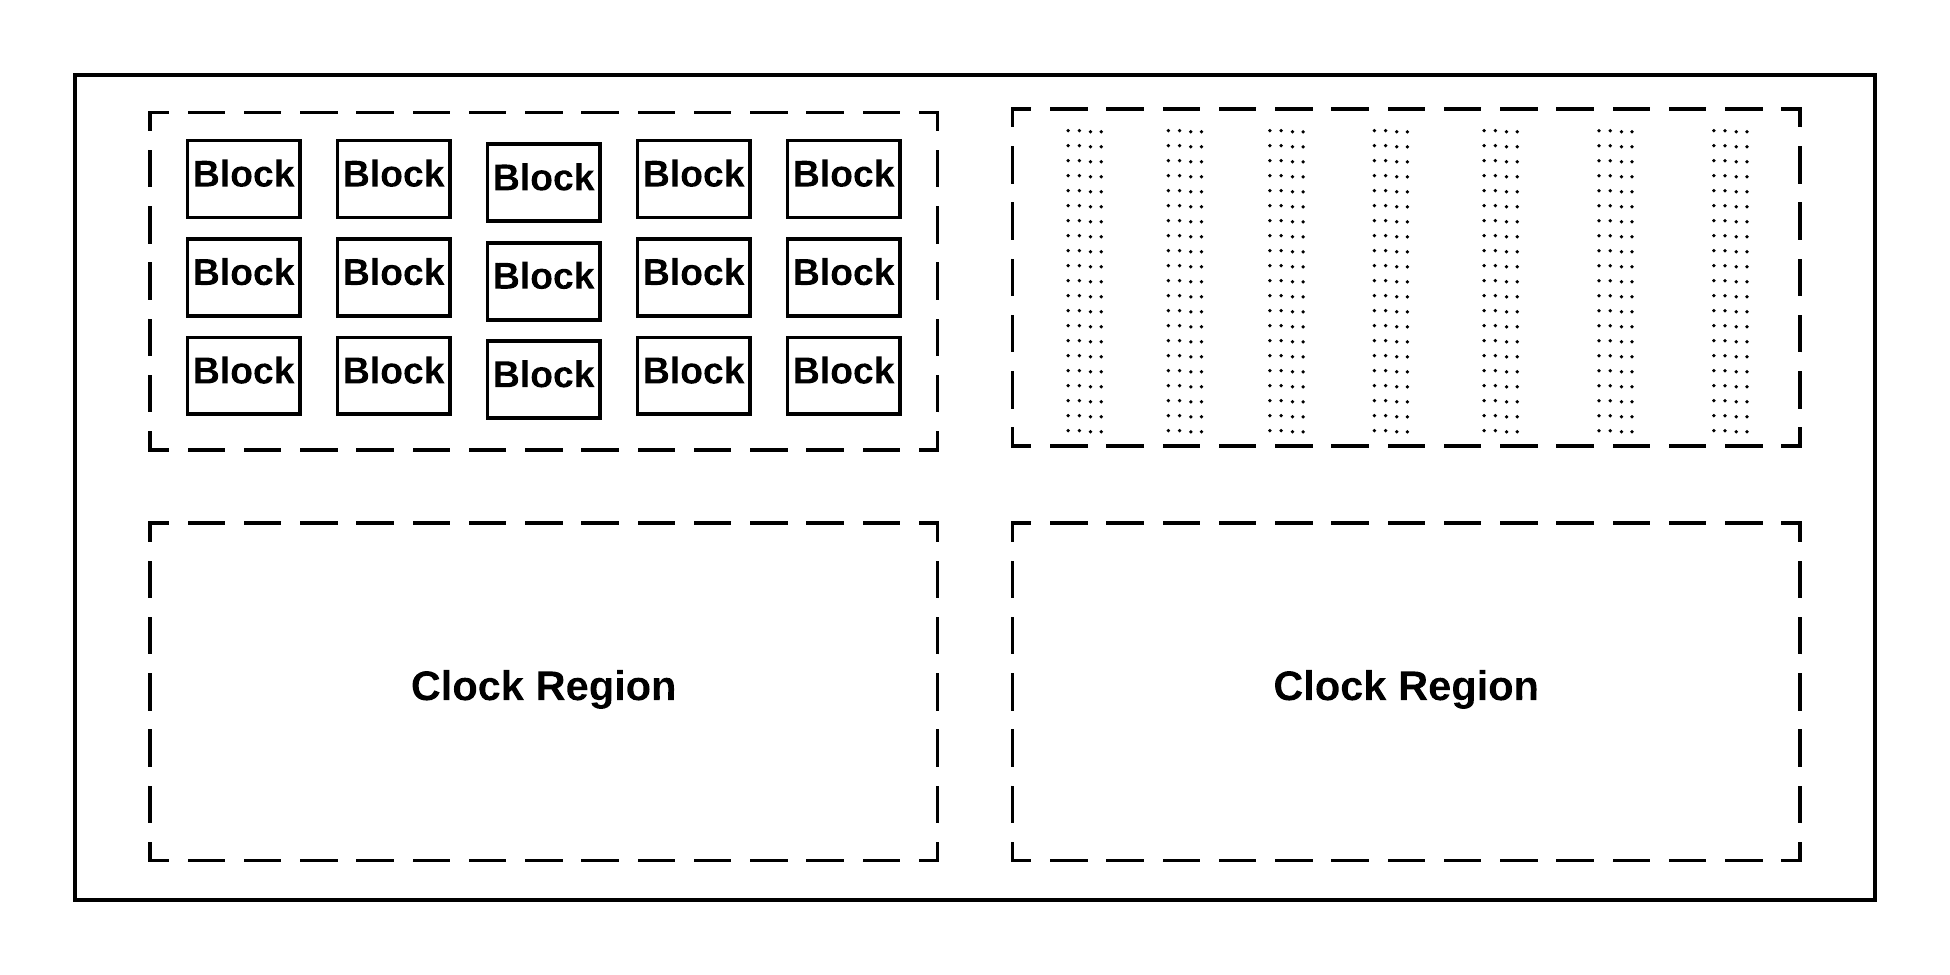
\includegraphics[width=1\linewidth]{figures/FPGA}
	\caption[Gate-Array of Block Columns Separated into Clock Regions]{Gate-Array of Block Columns Separated into Clock Regions}
	\label{fig:FPGA}
\end{figure}
A block is not a physical device but a conceptual grouping of tiles.
A block will consist of one or multiple tiles depending on its type.
A tile is a component specific to a particular function such as \acrfull{IO}, design logic, memory...etc but their detailed functionality can be configured by the user.
Though an \acrshort{FPGA} may have over one-hundred different types of tiles each column is comprised entirely by a single block type.
Columns are separated into regions shown by the dashed lines in Figure~\ref{fig:FPGA}.
These regions each use a separate clock mechanism and are referred to as ``Clock Regions''.


Figure~\ref{fig:column} depicts a \acrfull{CLB} column.
As mentioned, blocks may contain multiple tiles.
Each row in Figure~\ref{fig:column} (i.e. the interconnect/\acrshort{CLB} tile-pair) is a block. 
In this column the \acrshort{CLB} tile is the primary feature of each block, hence, it is referred to as a \acrshort{CLB} block.
Consequentially, since this column is made up of \acrshort{CLB} blocks it is referred to as a \acrshort{CLB} column.
A column is comprised of blocks stacked vertically.
In the case where blocks contains multiple tiles, columns can be thought to contain sub-columns.
The stack of interconnects can be considered the ``interconnect'' sub-column while the stack of \acrshort{CLB} tiles can be thought of as the \acrshort{CLB} sub-column.
Combined, the two sub-columns make up this \acrshort{CLB} column. 
\begin{figure}
\centering
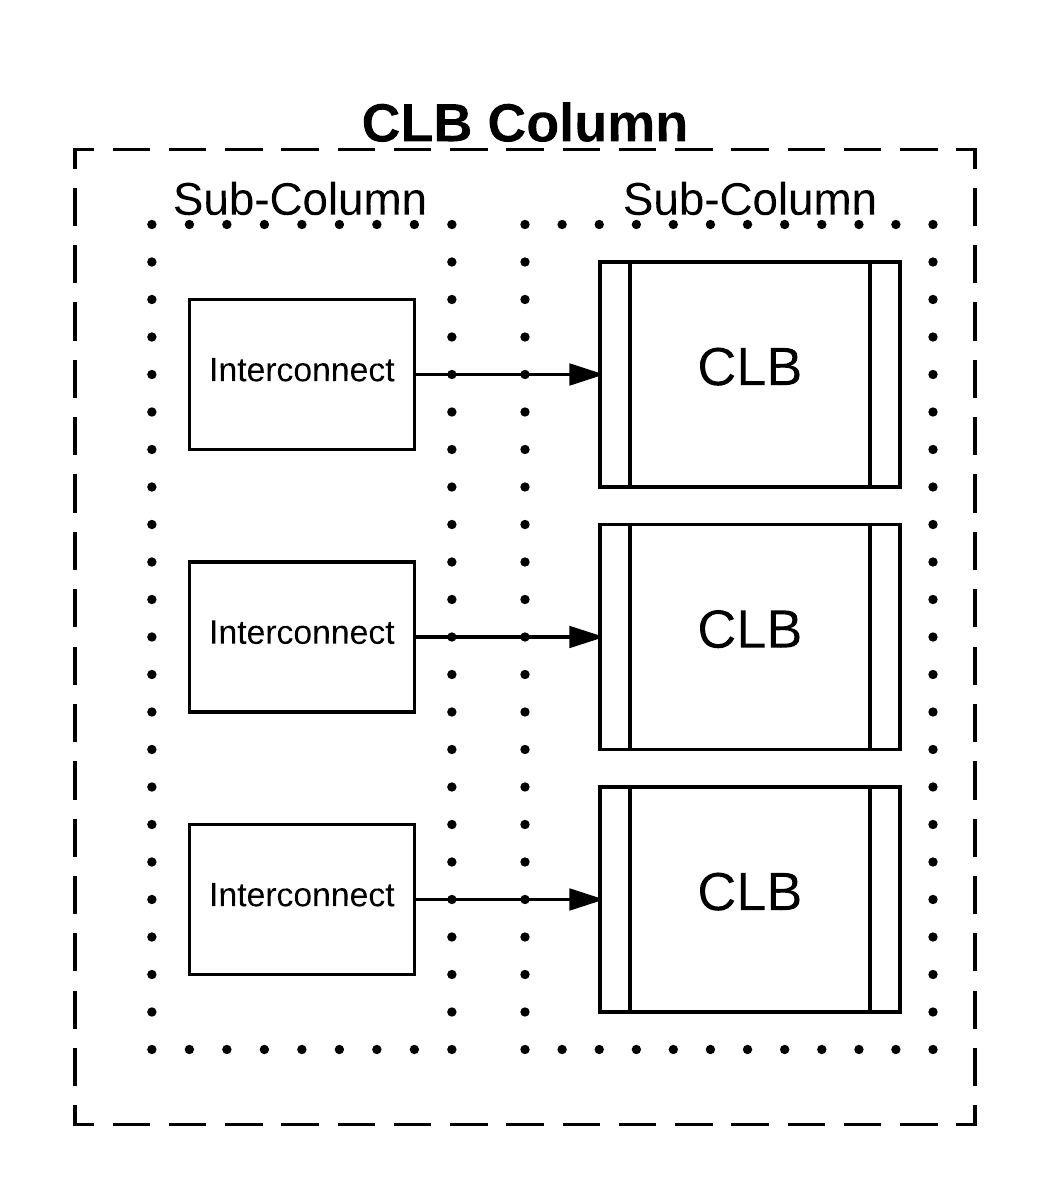
\includegraphics[width=0.7\linewidth]{Figures/column}
\caption[Column Composition]{Column Composition}
\label{fig:column}
\end{figure}
Though each tile has a designated purposes (ex. \acrfull{IO}, \acrfull{CL}, memory...etc) their functionality can be configured by the user; this is how designs are implemented on a device.
The configuration of each tile is dictated by the \gls{Bitstream}. 
\begin{figure}[h]
	\centering
	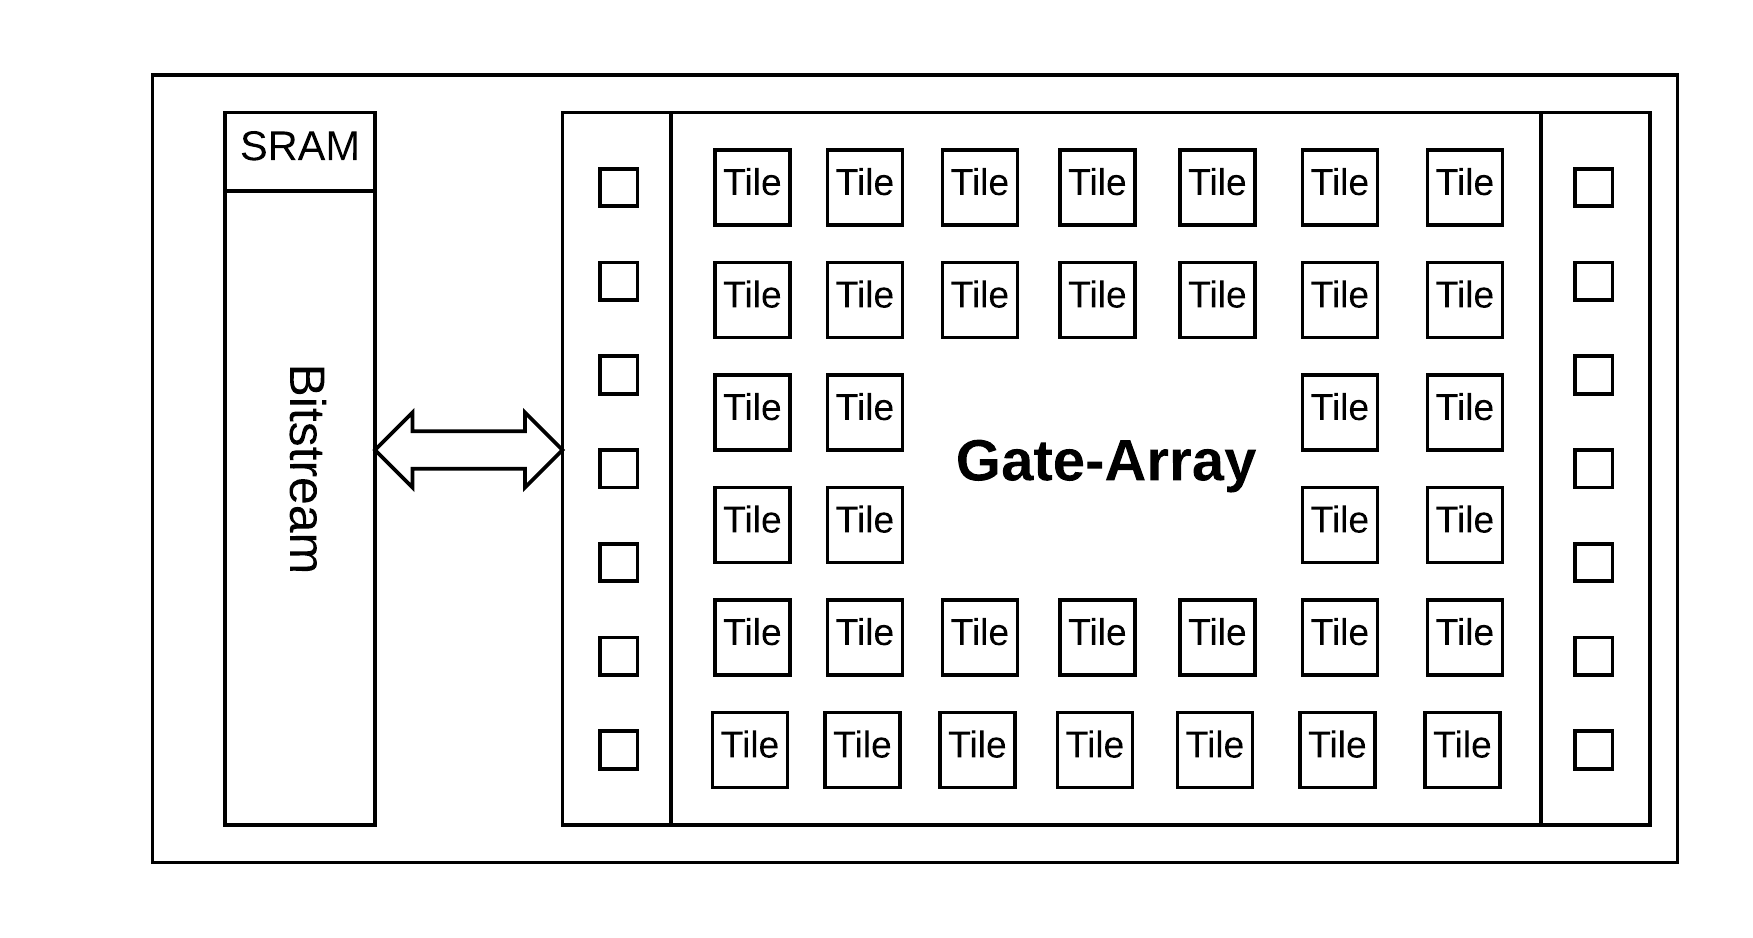
\includegraphics[width=0.9\linewidth]{Figures/architecture}
	\caption[FPGA Device Layout]{FPGA Device Layout}
	\label{fig:architecture}
\end{figure}

To improve performance the blocks of the gate-array are dynamic memory components.
A dynamic device is unable to retain the contents of its memory when it looses power.
To prevent having to plug in a device and download the configuration every time it is powered on, an external static memory device (i.e. retains its contents with loss of power) holds the \gls{Bitstream}. 
When an \acrshort{FPGA} is powered on the \gls{Bitstream} is loaded from the external memory (often \acrfull{SRAM}) into the gate-array, as can be seen in Figure~\ref{fig:architecture}.


%%%%%%%%%%%%%%%%%%%%%%%%%%%%%%%
\section{\gls{Bitstream} Extraction} \label{sec:bitstreamExtraction}
In order to detect any trojans in the \gls{target} device the configuration \gls{Bitstream} will need to be recovered.
As mentioned in section~\ref{sec:architectureAndConfig} the \gls{Bitstream} is stored in a memory unit external to the gate-array~\cite{virtex5ConfigGuide}.
All \Xilinx devices provide a feature known as \gls{Readback}.
There are two styles of \gls{Readback}; \gls{Readback} verify and \gls{Readback} capture.
The \gls{Readback} capture method provides a large quantity of debug information which is not needed; \gls{Readback} verify will be used.
\gls{Readback} verify is the process where the device is put into a ``frozen'' state during run-time and all of the configuration bits are returned from the gate-array to the \acrshort{SRAM}. 
The results can then be uploaded to a \acrfull{PC} for analysis.
This process overwrites the original frame data in the \acrshort{SRAM} with the values which actually configured the device. 
By using this method rather than simply reading the \acrshort{SRAM} it ensures that what is tested in section~\ref{sec:fpgaBitStream} is actually what configured the device.
This minimizes risk of tampered external memory units or configuration mechanics. 


%%%%%%%%%%%%%%%%%%%%%%%%%%%%%%%
\section{The \acrshort{FPGA} \gls{Bitstream} Analysis} \label{sec:fpgaBitStream}
The \Xilinx \gls{Bitstream} is a binary file composed of a series of 32-bit words organized into ``frames''.
A frame is a string of single bits that span from the top to the bottom of a clock region of a device as seen in the top-right quadrant of Figure~\ref{fig:FPGA}.
A frame affects every block in a column and multiple horizontally adjacent frames are required to configure an entire column.
Each frame is uniquely identified by a 32-bit address and is the smallest addressable element.
The composition of the frame address is fairly consistent across the \Xilinx catalog however there are small differences between device families.
The following is the structure of the Virtex-5 family frame address scheme according to~\cite{virtex5ConfigGuide}.
The make-up of a frame address is shown in Table~\ref{tbl:frameAddress}.
\begin{table}[h]
	\centering
	\caption{Frame Address}
	\label{tbl:frameAddress}
	\resizebox{\textwidth}{!}{
		\begin{tabular}{|c|c|c|c|c|c|c|c|c|c|c|c|c|c|c|c|c|c|c|c|c|c|c|c|c|c|c|c|c|c|c|c|}
			\hline
			\multicolumn{8}{|c|}{Unused} & \multicolumn{3}{c|}{BA} & T & \multicolumn{5}{c|}{Row Address} & \multicolumn{8}{c|}{Major Address} & \multicolumn{7}{c|}{Minor Address} \\ \hline
			31 & 30 & 29 & 28 & 27 & 26 & 25 & 24 & 23 & 22 & 21 & 20 & 19 & 18 & 17 & 16 & 15 & 14 & 13 & 12 & 11 & 10 & 9 & 8 & 7 & 6 & 5 & 4 & 3 & 2 & 1 & 0 \\ \hline
			0 & 0 & 0 & 0 & 0 & x & x & x & x & x & x & x & x & x & x & x & x & x & x & x & x & x & x & 0 & 0 & 0 & 0 & 0 & 0 & 0 & 0 & 0 \\ \hline
		\end{tabular}		
	}
\end{table}

The \acrfull{BA} identifies the block type.
\begin{itemize}
	\item BA 0: Logic type.
	\item BA 1: \acrfull{BRAM}.
	\item BA 2: \acrshort{BRAM} Interconnect.
	\item BA 3: \acrshort{BRAM} non-configuration frame.
\end{itemize}
The logic block contains the columns which provides the primary configuration for the device (\acrshort{CLBs}, \acrshort{IOBs}... etc).
The \acrshort{BRAM} columns initialize the memory for the device while the \acrshort{BRAM} Interconnect columns configure how the logic of the design interacts with the \acrshort{BRAM}.

%In the case of the Virtex-5 family each clock region is composed of twenty blocks in a column separated by a horizontal clock bus as shown in Figure~\ref{fig:RowOrder}.
\begin{figure}[h]
\centering
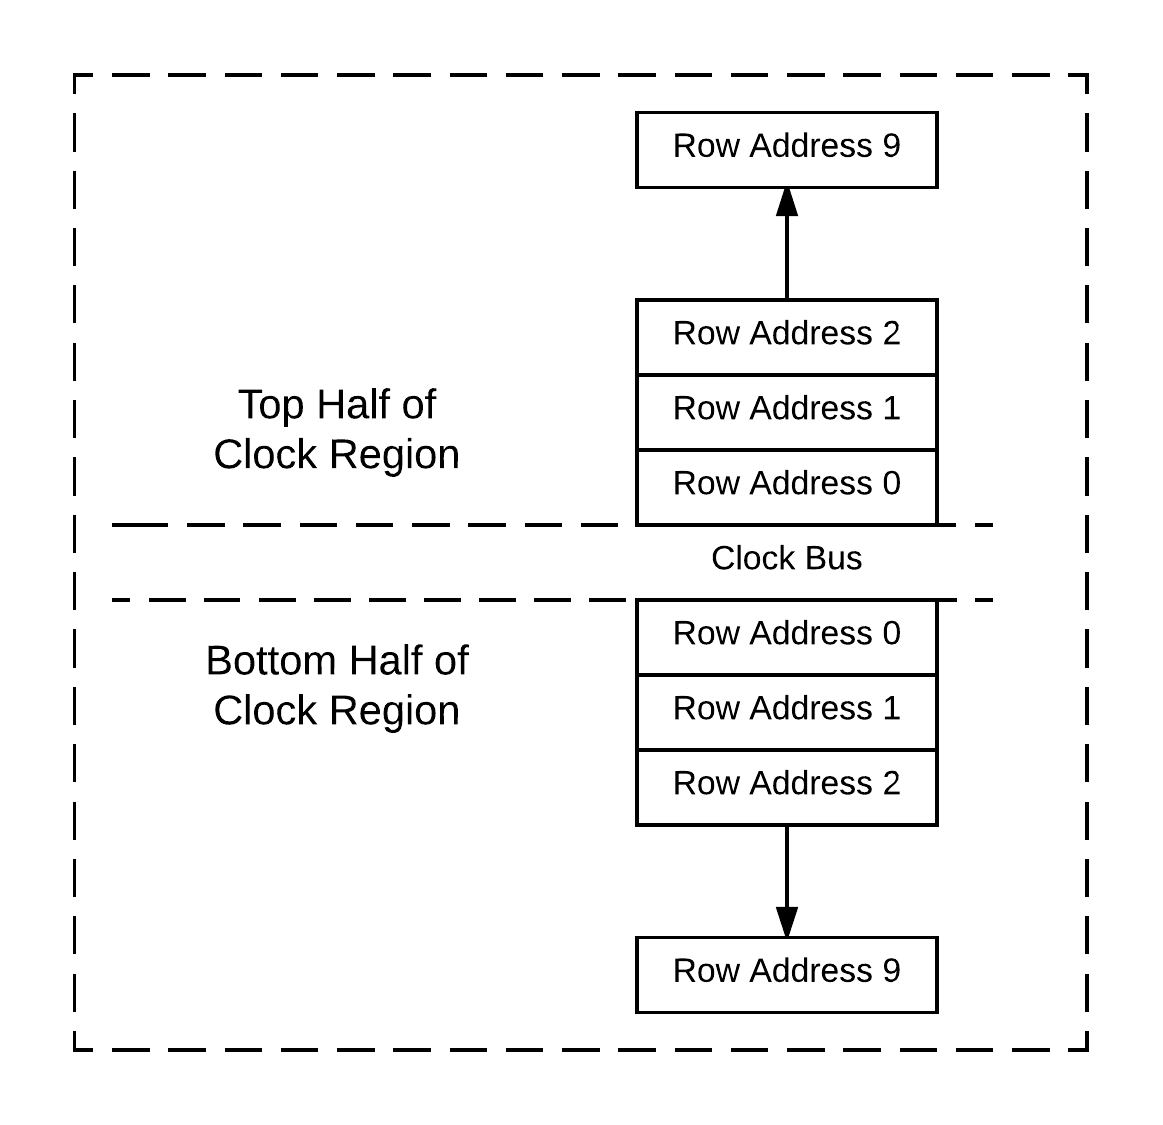
\includegraphics[width=.7\linewidth]{Figures/RowOrder}
\caption[Row Order of Virtex-5 Clock Region]{Row Order of Virtex-5 Clock Region}
\label{fig:RowOrder}
\end{figure}
Each clock region is given a row value in its address that increments away from the center of the device starting at 0. 
The frame address includes a Top indicator bit in position 20 that indicates whether the specified row is above or below the center of the device~\cite{virtex5ConfigGuide}.
The major address specifies the column within the row.
These addresses are numbered from left to right and begin at 0.
The minor address indicates the frame number within a column. 
Table~\ref{tbl:minorAddressNumbers} provides the number of frames per column type.
\begin{table}[h!]
	\centering
	\caption{Number of Frames (minor addresses) per Column~\cite{virtex5ConfigGuide}}
	\label{tbl:minorAddressNumbers}
	\begin{tabular}{|c|c|}
		\hline
		Block             & Number Of Frames \\ \hline
		CLB               & 36               \\ \hline
		DSP               & 28               \\ \hline
		\acrshort{BRAM}   & 30               \\ \hline
		IOB               & 54               \\ \hline
		Clock             & 4                \\ \hline
	\end{tabular}
\end{table}
As described in section~\ref{sec:architectureAndConfig} a block may contain multiple tiles.
In a \acrshort{CLB} column a block consists of an interconnect tile, also known as a \acrfull{SM} and a \acrshort{CLB}.
Frames are numbered from left to right, starting with 0. 
For each block, except in a clock column, frames numbered 0 to 25 access the interconnect tile for that column. 
For all blocks, except the \acrshort{CLB} and the clock column, frames numbered 26 and 27 access the Interface for that column. 
All other frames are specific to that block~\cite{virtex5ConfigGuide}.
To further understand how frames configure tiles a mapping must be made between each frame and the corresponding tile.
This is described in section~\ref{sec:tileMapping}.

%%%%%%%%%%%%%%%%%%%%%%%%%%%%%%%
\section{Component Mapping} \label{sec:tileMapping}
The \NameNoPeriod employs a method referred to as Component Mapping to create a mapping between each word in a configuration frame and the component on the device that it configures.
This information is not publicly released by \Xilinx as a means of providing security through obscurity.

\subsection{Frame to Column Mapping}
The configuration \gls{Bitstream} is stored in an external memory device as described in section~\ref{sec:architectureAndConfig}.
When powered-on the \gls{Bitstream} is transmitted in frame address order to populate the dynamic memory in the tiles of the gate-array.
The frame addressing scheme describes where in the gate-array the frame is destined fairly directly.
Frames with a \acrshort{BA} value of 1 are clearly destined to configure the \acrshort{BRAM} and do not need further analysis for the purposes of this method.
Frames with a \acrshort{BA} value of 0 or 2 must be mapped more finitely.
The row address specifies which row of clock-regions the frame is destined.
Figure~\ref{fig:FPGA} shows four clock regions organized into two rows. 

As an example the Virtex-5 240T has 12 rows; its row address spans from 0-5 and the Top bit in the address indicates whether it is in the top or bottom half of the device in accordance with Figure~\ref{fig:RowOrder}.
Once the correct clock region is discerned the major address is used to determine which column the frame configures.
The major address begins at 0 on the left and counts up towards the number of columns in the row.
Finally, the minor address is used to determine which sub-column has been modified according to Table~\ref{tbl:frameAddress}.
\subsection{Word to Block Mapping}
In the case of Virtex-5 devices a frame is composed of 41 words that can be thought of as a vertical stack that aligns with a column.
As described in section~\ref{sec:fpgaBitStream} a row consists of a stack of basic blocks; there are 20 \acrshort{CLB} blocks per column, 40 \acrshort{IOB}s, 4 \acrshort{BRAM}...etc for Virtex-5 devices.
\begin{figure}[h]
	\centering
	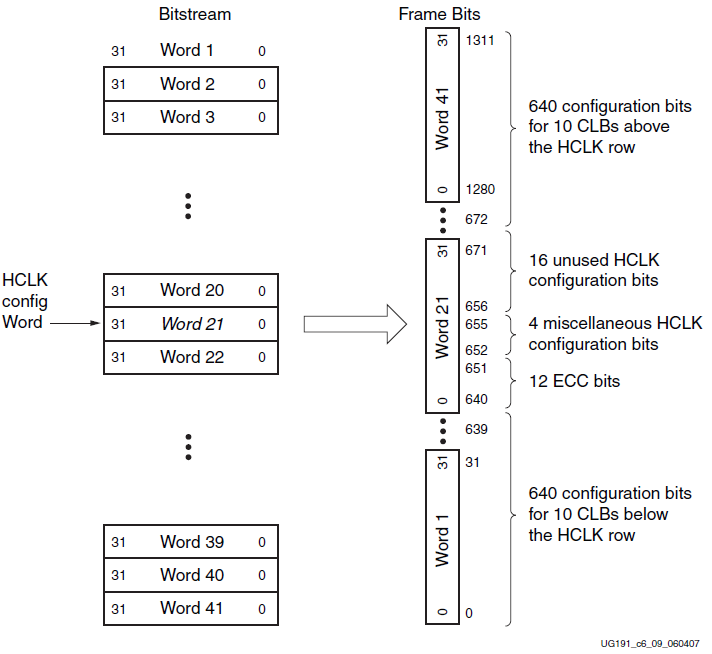
\includegraphics[width=0.9\linewidth]{Figures/frameTileMap}
	\caption[Configuration Words in the Bitstream~\cite{virtex5ConfigGuide}]{Configuration Words in the Bitstream~\cite{virtex5ConfigGuide}}
	\label{fig:frameTileMap}
\end{figure}
As can be seen in Figure~\ref{fig:frameTileMap} the central word in a frame configures the horizontally running clock bus.
The remaining words are used to configure the blocks in the column.
The purpose of the central word in the column is known to be mapped to the clock bus.
For the purposes of the following computations it is considered removed from the frame.
From this, equation~\ref{eqn:numWordsPerBlock} can be deduced which is used to compute the number of 32-bit words that span each block.
\begin{equation} \label{eqn:numWordsPerBlock}
n = (W - C) + B
\end{equation}
\ConditionSize
where:
\begin{conditions}
	n     &  Number of Words per Block \\
	W     &  Number of 32-bit words per frame \\   
	C     &  Number of clock words per frame \\
	B     &  Number of blocks per column
\end{conditions}
\normalsize
As shown in Figure~\ref{fig:frameTileMap} words are addressed from the ``top'' of a device down.
Equation~\ref{eqn:getTileNumber} can be used to map a particular word in a frame to a block on the device.
\begin{equation} \label{eqn:getTileNumber}
i = B - \floor*{\frac{w}{n}}
\end{equation}
\ConditionSize
where:
\begin{conditions}
	i     &  Word Number in frame\\
	B     &  Number of blocks per column \\
	w     &  Word number \\
	n     &  Number of Words per Block 
\end{conditions}
\normalsize
With equations~\ref{eqn:numWordsPerBlock} and~\ref{eqn:getTileNumber} it is now possible attribute any modifications in the \gls{Bitstream} to its corresponding block.

\section{Determining Trojan Attributes} \label{sec:trojanAttributes}
The complexity of \acrlong{IC} designs and their corresponding trojans requires a more human-friendly scope.
The taxonomy described in Chapter~\ref{chapter:hardwareTrojans} provides a series of thirty-three attributes which a trojan may or may not posses.
These attributes allow us to readily describe, interpret and discuss trojans in a more comfortable and useful way.
To employ this taxonomy a trojan must be analyzed; characteristics observed can either infer or provide direct evidence of possession of attributes. 
Though it is desirable to be able to observe and directly extract the attributes a trojan possesses it is not always possible. 
In~\cite{samerAttribute} a matrix, $\mathbf{R}$, is provided which describes the relationships between each of the thirty-three attributes in the taxonomy.
When it is not possible to directly determine the presence of certain attributes, this relation matrix is used to infer their existence.
The analysis stage of the automated trojan detection technique provided by this work begins by extracting those attributes that are directly observable then using matrix $\mathbf{R}$ to infer the existence of the remainder. 
\subsection{Extraction Methods} \label{sec:directExtractionMethods}
\subsubsection{Observed Location Attributes}
The presence of attributes in the \textit{Location} category are directly observable from the results of the component mapping method described in section~\ref{sec:tileMapping}.
\Xilinx tiles conform to purpose-specific groups or block types which were discussed in section~\ref{sec:fpgaBitStream}.
These block types contain sub-types that perform actions which pertain to the \textit{Location}, category. 
\begin{enumerate}
	\item The \textbf{Processor} attribute pertains to the core functionality of the design logic. It can be awarded for presence of a modified \acrshort{CLB} tile or Interconnect tile.
	\item The \textbf{Memory} attribute can be awarded for the presence of modified \acrshort{BRAM} components.
	\item The \textbf{\acrshort{IO}} attribute can be awarded for presence of modified \acrshort{IOB} tiles.
	\item The \textbf{Power Supply} attribute can be awarded for the presence of modified interface or configuration tiles.
	\item The \textbf{Clock Grid} attribute can be awarded for modified clock tiles.
\end{enumerate}
\subsubsection{Scatter Score Method} \label{sec:scatterScore}
The gate-array configuration of components in \Xilinx \acrshort{FPGA}s allows for an analytical method of determining attributes in the \textit{Physical Layout} category.
The "Scatter Score" method uses the grid coordinates of components to derive a numerical score rating for the size, position, and augmentation of configured tiles.
Tiles are assigned global coordinates that represent their horizontal and vertical positions within the gate array denoted $x$ and $y$ respectively. 
These values can then be used to strongly infer the presence of \textit{Physical Location} attributes.

The golden chip is first analyzed.
The set of all tiles which are configured in the golden design is found and a series of numerical descriptors are computed.
\begin{equation} \label{eqn:numConfiguredTiles}
n = \sum_{x = 0}^{X}\sum_{y = 0}^{Y}T_{xy}
\end{equation}
\ConditionSize
where:
\begin{conditions}
	n     &  Number of all \textbf{configured} tiles \\
	X     &  The column width of the gate-array \\   
	Y     &  The number of rows of the gate-array \\
	T     &  A configured tile
\end{conditions}
\normalsize

\noindent\begin{minipage}{.5\linewidth}
	\begin{equation} \label{eqn:xAverage}
	a_x = \frac{1}{n}\sum_{x=0}^{n}T_x
	\end{equation}
\end{minipage}%
\begin{minipage}{.5\linewidth}
	\begin{equation} \label{eqn:yAverage}
	a_y = \frac{1}{n}\sum_{y=0}^{n}T_y
	\end{equation}
\end{minipage}
\\
\noindent\begin{minipage}{.5\linewidth}
	\begin{equation} \label{eqn:stdDevX}
	\sigma_x = \sqrt{\frac{1}{n}\sum_{x = 0}^{X}(x_i - a_x)^2)}
	\end{equation}
\end{minipage}%
\begin{minipage}{.5\linewidth}
	\begin{equation} \label{eqn:stdDevY}
	\sigma_y = \sqrt{\frac{1}{n}\sum_{y = 0}^{Y}(y_i - a_y)^2)}
	\end{equation}
\end{minipage}

\ConditionSize
where:
\begin{conditions}
	$$a_x$$     &  The average x coordinate of configured tiles \\   
	$$a_y$$     &  The average y coordinate of configured tiles \\
	$$T_x$$     &  The x coordinate of a configured tile \\
	$$T_y$$	    &  The y coordinate of a configured tile \\
	$$\sigma_x$$ & The standard deviation of the x coordinate of configured tiles \\
	$$\sigma_y$$ & The standard deviation of the y coordinate of configured tiles
\end{conditions}
\normalsize
Equations~\ref{eqn:xAverage} and~\ref{eqn:yAverage} are used to create a rating known as the \gls{positionMedian} in Equation~\ref{eqn:positionMedian}.
The \gls{positionMedian} value provides a simple descriptor for where in the gate array the design is centralized.
The \gls{scatterScore} in Equation~\ref{eqn:scatterScore} describes how spread out or, \textit{clustered} the design is.

\noindent\begin{minipage}{.5\linewidth}
	\begin{equation} \label{eqn:positionMedian}
	M_{xy} = (a_x,~a_y)
	\end{equation}
\end{minipage}%
\begin{minipage}{.5\linewidth}
	\begin{equation} \label{eqn:scatterScore}
	S_{xy} = (\sigma_x,~\sigma_y)
	\end{equation}
\end{minipage}
\ConditionSize

where:
\begin{conditions}
	$$M_{xy}$$     &  The \gls{positionMedian} \\   
	$$S_{xy}$$     &  The \gls{scatterScore}
\end{conditions}
\normalsize

The results of the component mapping method described in section~\ref{fig:frameTileMap} are used to generate the set of all tiles reconfigured by the trojan.
The set of reconfigured tiles can be said to contain three subsets: the subset of tiles activated by the trojan, those deactivated and those modified. 
The results of the golden design analysis, the subsets, and the numeric descriptors can be used to discern which of the \textit{Physical Location} attributes the trojan possesses. 
The \textit{Physical Location} category contains six attributes.
These six can be considered three pairs; a trojan exhibits one attribute from each pair. 
\begin{enumerate}
	\item \textbf{Large or Small} (attributes 23 or 24): According to~\cite{samerAttribute}, small trojans are defined as those that are nearly impossible to detect via power consumption. From this it can be said that ``small'' trojans occupy minimal resources. Trojans where the number of reconfigured tiles is less than 5\% of the number of tiles in the golden design are considered small. Other wise they are attributed as large.
	\item \textbf{Changed Layout or Augmented} (attributes 25 or 26): A ``changed layout'' trojan is such that only tiles that are configured by the golden design are reconfigured. An augmented trojan is where additional layout is added. The presence of ``activated'' or ``deactivated'' tiles indicates an augmented trojan. 
	\item \textbf{Clustered or Distributed} (attributes 27 or 28): The trojan is considered to be clustered when the standard deviation of the reconfigured tile positions is less than 15\%; distributed otherwise.
\end{enumerate}
\subsubsection{Insertion and Abstraction Attributes}
The linear nature of the manufacturing life-cycle implies a propagation of effects.
Design decisions, flaws and improvements affect later stages.
As discussed in section~\ref{sec:methodology}, for the purposes of this automated \acrshort{FPGA} trojan detection method it is assumed that the only non-trustworthy stage in the life-cycle is fabrication.
In other words, the trojan was inserted in the third-party fabrication stage.
Due to the propagating nature of the life-cycle the effects of the modifications made in the fabrication stage (attribute 3) are felt in the testing (attribute 4) and assembly (attribute 5) stages.
Hence, due to the assumptions made in this method it can be said that this trojan possesses insertion category attributes 3, 4 and 5.

The abstraction category pertains to the level at which a trojan resides~\cite{killSwitch, regionBasedApproach}.
Due to the nature of \acrshort{FPGA} design a few additional assumptions can be made when selecting abstraction category attributes.
\acrfull{HDL} is used to generate a "programming", or "configuration" file which is downloaded into the \acrshort{FPGA}.
The configurable functionality is dictated by this file. 
The hardware of an \acrshort{FPGA} chip can be modified to hide trojans at a lower abstraction level.
The detection of such trojans requires advanced reverse engineering techniques and is beyond the scope of this method.
Hence, it can be said that trojans discovered by this method are not able to obtain abstraction category attributes that pertain to the physical hardware of a chip.
This removes the possibility of \textit{Logic} (attribute 9), \textit{Transistor} (attribute 10), and \textit{Physical} (attribute 11).
The possession of the remaining abstraction category attributes are determined by analysis of the relation matrix discussed in section~\ref{sec:matrixUse}.
\subsection{Relation Matrix Use} \label{sec:matrixUse}
The relation matrix $\mathbf{R}$ provided in chapter~\ref{chapter:hardwareTrojans} can be summarized by a series of submatrices.
\[
\newcommand\scalemath[2]{\scalebox{#1}{\mbox{\ensuremath{\displaystyle #2}}}}
\mathbf{R} =\left[
\scalemath{1.1}{
	\begin{array}{l*{3}{c}}
	\mathbf{R_1} ~ & ~ \mathbf{R_{12}} ~ & ~ 0 ~  &  ~ 0   \\
	0         & \mathbf{R_2}      &\mathbf{R_{23}}       & ~ 0 \\
	0          & 0           & \mathbf{R_3}          & ~ \mathbf{R_{34}} \\
	0          & 0           & 0                & ~ \mathbf{R_4} \\
	\end{array}
}
\right]
\label{R}
\]
Each submatrix is a matrix of binary values which describe the relationship between two attributes.
Refer to section~\ref{sec:trojanBackGround} for a detailed description.
Submatrix $\mathbf{R_{34}}$ relates the \textit{Location} category attributes to \textit{Properties} attributes. 
Since the \textit{Location} attributes are directly observable they can be used to generate a list of \textit{Property} attributes which the trojan may possess. 
This list is compared to results generated by any additional property attribute extraction methods, such as the \textit{Scatter Score} method described in section~\ref{sec:scatterScore}.

Once a list of \textit{Property} attributes has been solidified submatrix $\mathbf{R_{23}}$ is used to infer the \textit{Abstraction} category attributes. 
As mentioned in section~\ref{sec:directExtractionMethods} \textit{Abstraction} category attributes nine, ten and eleven are assumed inaccessible.
Attributes six, seven and eight can be inferred based on the presence \textit{Property} attributes. 

\section{Coverage Rating} \label{sec:automationCoverage}
As described in section~\ref{sec:techniqueEvaluation} a hardware trojan detection method can be assigned a coverage vector which describes it strength.
Referring to the tables presented in~\cite{samerDissertation} the $I$ and $C$ values for each of the eight categories can be found.
\NameNoPeriod is found to have the coverage rating shown in table~\ref{tbl:nameCoverageRating}.
\begin{table}[h]
	\centering
	\caption{Coverage Rating of \Name}
	\label{tbl:nameCoverageRating}
	\begin{tabular}{|c|c|c|c|c|c|c|c|c|c|c|c|c|c|c|c|}
		\hline
		\multicolumn{8}{|c|}{Parameters ($I_P$)} & \multicolumn{8}{c|}{Coverage ($C_P$)} \\ \hline
		$I_R$ & $I_A$ & $I_E$ & $I_L$ & $I_F$ & $I_C$ & $I_P$ & $I_O$ & $C_R$ & $C_A$ & $C_E$ & $C_L$ & $C_F$ & $C_C$ & $C_P$ & $C_O$ \\ \hline
		3 & 5 & F & 3 & 3 & 7 & 8 & V & 3 & 5 & 9 & 3 & 3 & 7 & 6 & 5 \\ \hline
	\end{tabular}
\end{table}